\chapter{Implementation}
\label{chapter:implementation}


TODO Some text here for latex placement


% ###############################################################
\section{Upgrading Kubric to use Blender to version 3.2}
\label{sec:upgrading-kubric}

The procedurally generated graphics pipeline is implemented in Blender as a feature called "Geometry Nodes". It is a visual and node-based programming environment that allows 3D artists to create and manipulate different attributes of an object's geometry. Operations on geometry made in this way include arithmetic and vector math, conditional logic, curve resampling, mesh triangulation, material selection, ray tracing and object instancing.

The "Geometry Nodes" feature was added in Blender 2.92, reworked in Blender 3.0 to make designing Geometry Node Groups more abstract and functional. Later releases have added more node types and performance improvements. We chose to make use of Blender version 3.2 as the render engine. This required updating the Kubric build process and resolving any breaking changes.

TODO references for the versions above
\footnote{\url{https://wiki.blender.org/wiki/Reference/Release_Notes/2.92/Geometry_Nodes}}
\footnote{\url{https://wiki.blender.org/wiki/Reference/Release_Notes/3.0/Nodes_Physics}}
\footnote{\url{https://wiki.blender.org/wiki/Reference/Release_Notes/3.1/Nodes_Physics}}
\footnote{\url{https://wiki.blender.org/wiki/Reference/Release_Notes/3.2/Nodes_Physics}}

TODO DIFF DOCKER IMAGES CODE EXTRACTS FROM GIT
TODO Docker Build explanations

The Docker Build process can also be used for other purposes, such as installing assets or Blender Plugins. An example of Blender Plugin installation is found in the next section.


% ###############################################################
\section{Saving and Restoring Blender Geometry Nodes}
\label{sec:save-restore-blender-geometry}

In the first section of this chapter we discussed how the Geometry Nodes in Blender is a new and actively developed feature. This means some operations cannot be achieved in a straight-forward fashion. This includes saving, restoring and transferring Geometry Nodes between Blender scenes.

In Blender 3.2 there is no direct way to import Geometry Node objects from another Blender project. However, imported Blender objects will keep all their linked Geometry Nodes objects, and all the Materials and Node Groups that are recursively linked by the first-order objects. This feature can be exploited to save and restore Geomtry Node Groups, by using a dummy object to store the geometry.

TODO code extract for save/restore geometry

This logic is used in the project for incremental Geometry Node Group development: the user can open the Blender Geometry Node editor, make changes, save the file, and re-run the save/restore script to use the new version in the scene generation in the full scene.

TODO simple diagram with edit-save-restore-recreate loop


% ###############################################################
\section{Downloading Geographic Data}
\label{sec:dowonload-geo-data}

As stated in the previous chapter, the first stage of the pipeline is concerned with collecting all geographic data required for a 3D scene at a chosen geographic location. To aid in accessing public data from GIS services, we use the BlenderGIS Plugin \footnote{\url{https://github.com/domlysz/BlenderGIS}}.

TODO Docker Build explanation of download + install plugin
TODO python code to activate plugin
TODO example screenshots in appendix for manual process
TODO python script to automate


% ###############################################################
\section{Combining Levels of Detail}
\label{sec:combine-levels-of-detail}

The geographic data aggregated by the BlenderGIS Plugin is stored in a number of Blender files, one for every zoom level. These assets must be combined into a single terrain object, with the scene action happening at the center of the smallest tile.

In addition to the reconciliation of the different level of details for the same terrain, this step must also reconcile the different types of data obtained from different sources. For example, the SRTM height map information does not perfectly match the road position at every point. To resolve this, a height adjustment step is made on both objects: the road track is wrapped to the terrain on the Z axis, and the terrain is flattened in the area immediately around the road track. A similar computation is made in parallel for all the other assets: rail tracks, urban zones, and building perimeters.

Finally, this step ensures adequate tessellation of the ground object. More detailed polygons are generated in the areas immediately around the roads, rails and buildings, and less accurate geometry is used everywhere else. This keeps the memory usage within a manageable level.

TODO Some text here for latex placement

\begin{figure}[H]
    \centering
    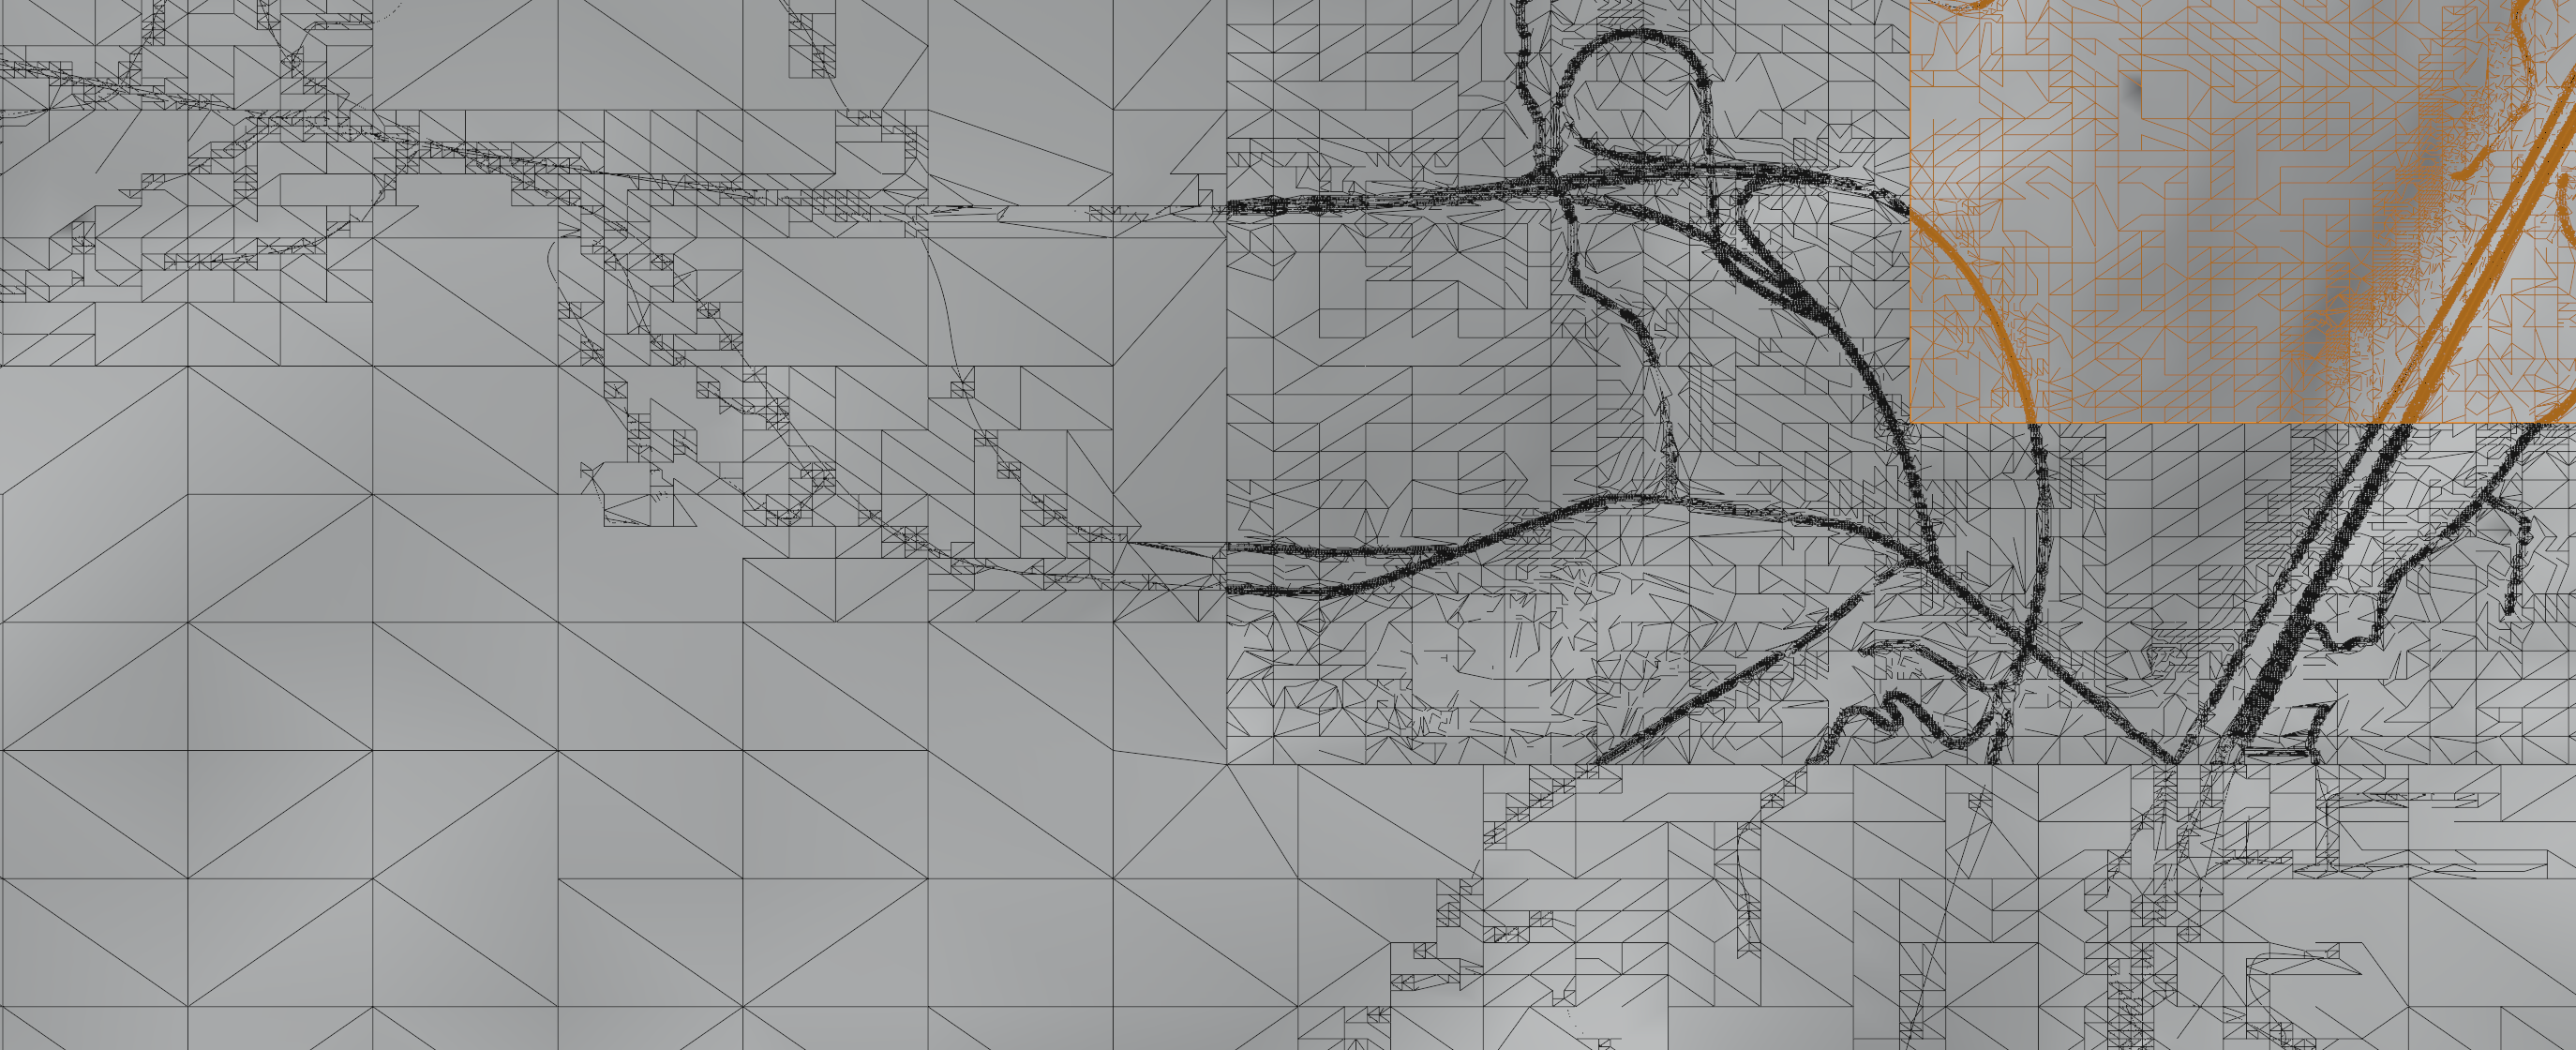
\includegraphics[width=14.5cm]{src/img/pic/pic-1 blender screenshot sat levels of detail.png}
    \caption{Different levels of detail }
    \label{fig:impl-levels-of-detail}
\end{figure}

TODO Some text here for latex placement

\begin{figure}[H]
    \centering
    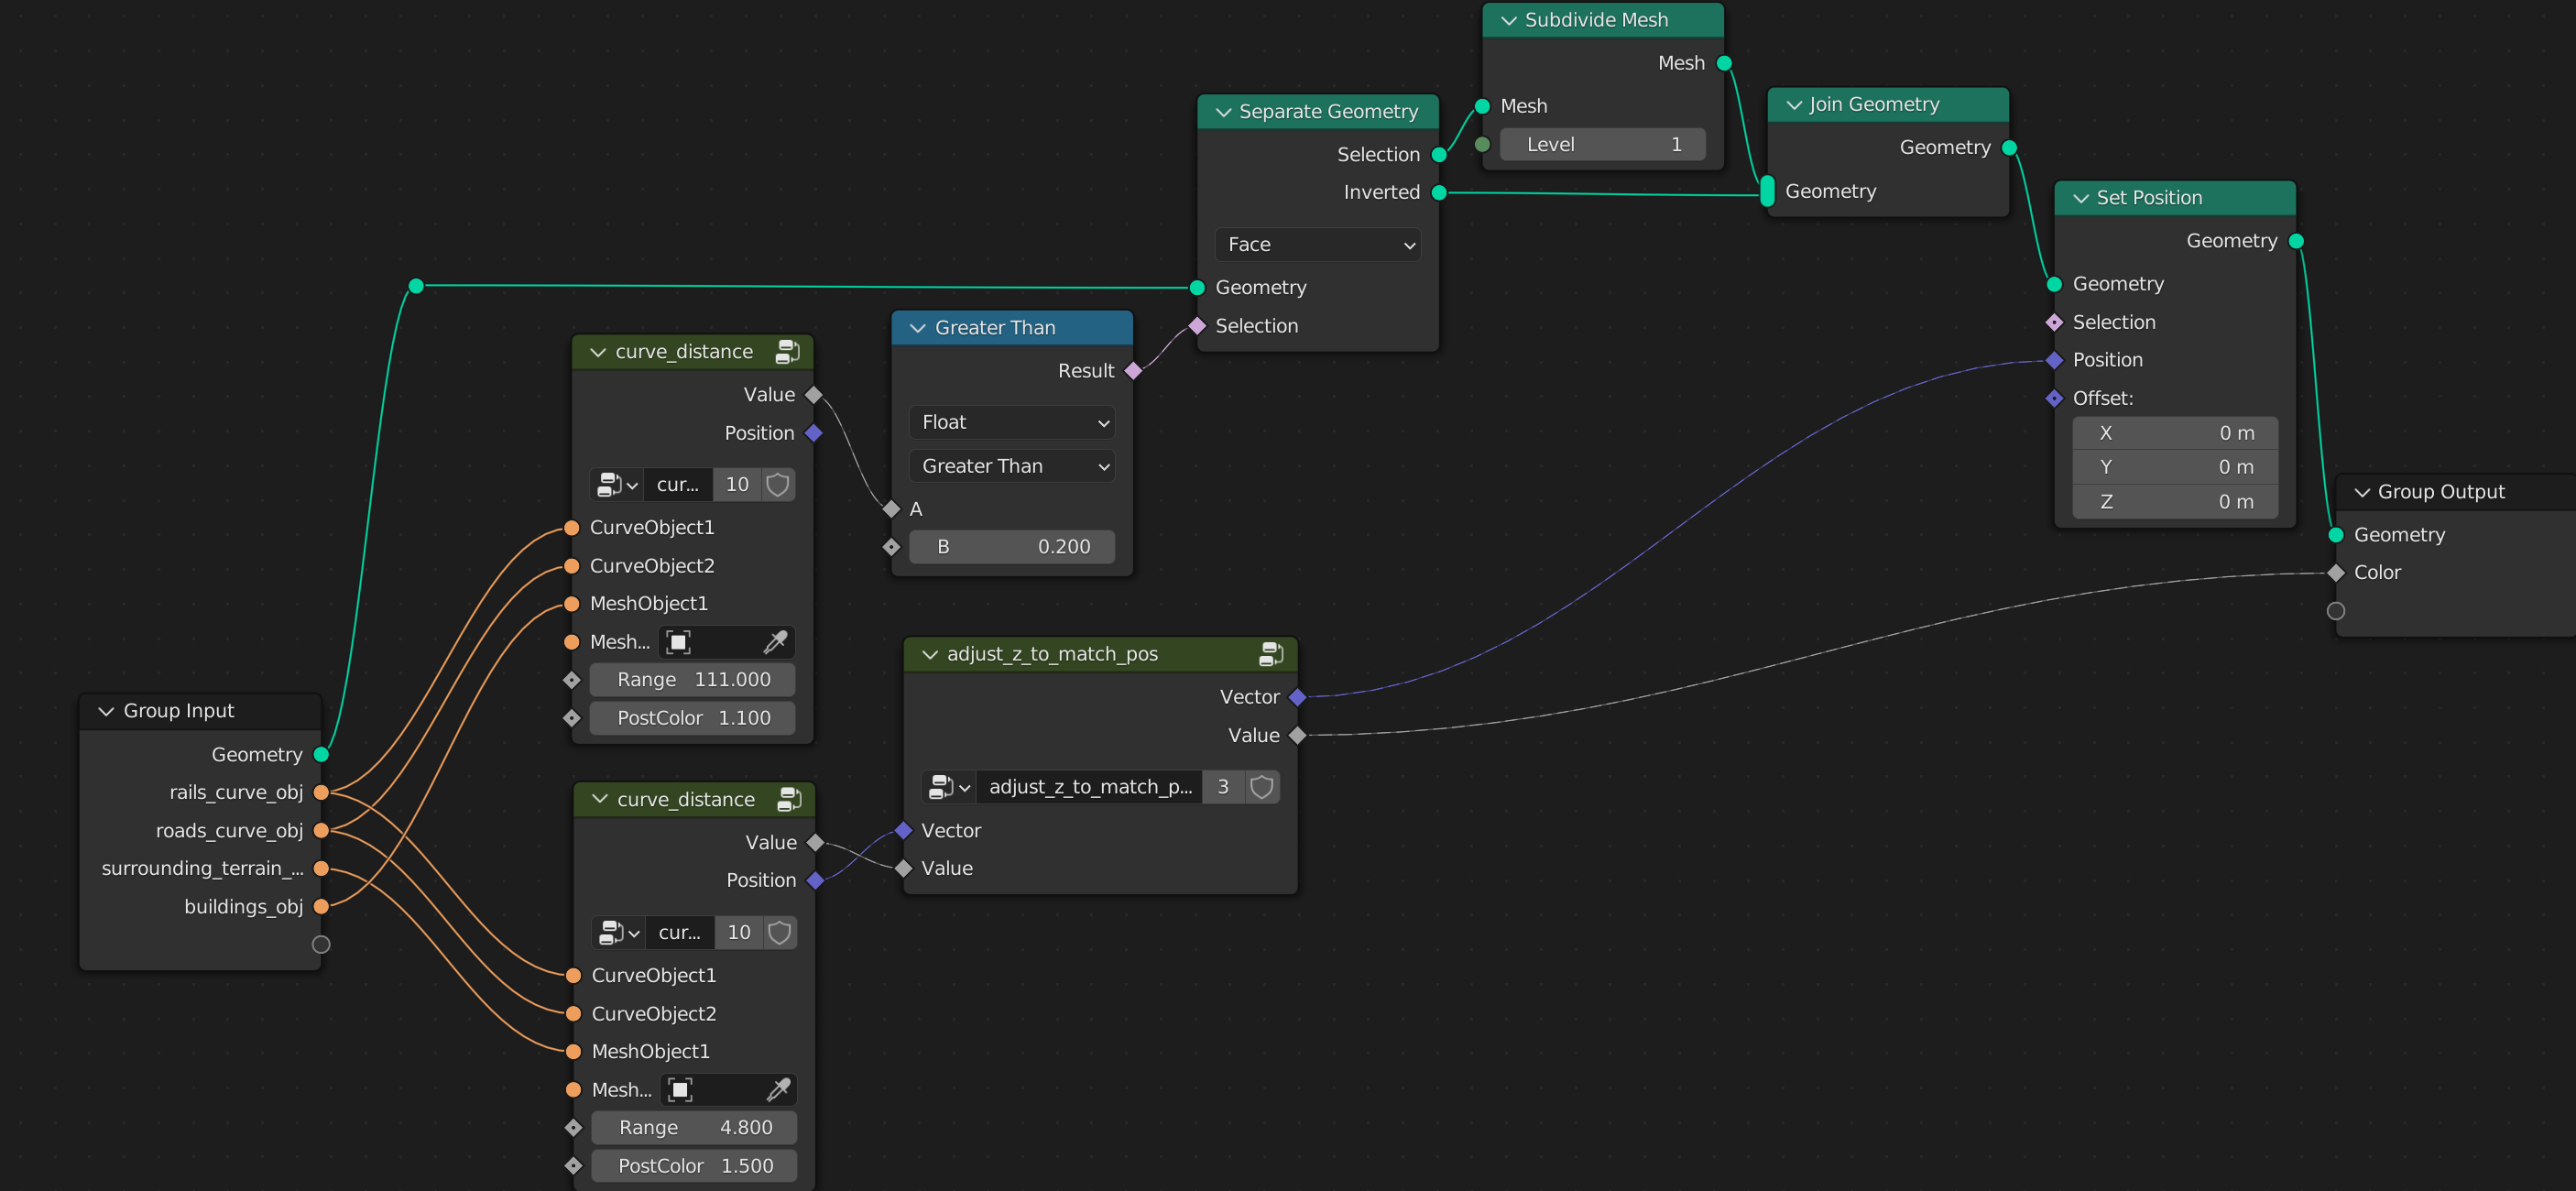
\includegraphics[width=14.5cm]{src/img/pic/pic-2 screenshot of blender adjust terrain geometry node.png}
    \caption{Geometry Node Implementation for terrain height adjustment and tessellation}
    \label{fig:impl-geom-nodes-terrain}
\end{figure}


TODO Some text here for latex placement


\begin{figure}[H]
    \centering
    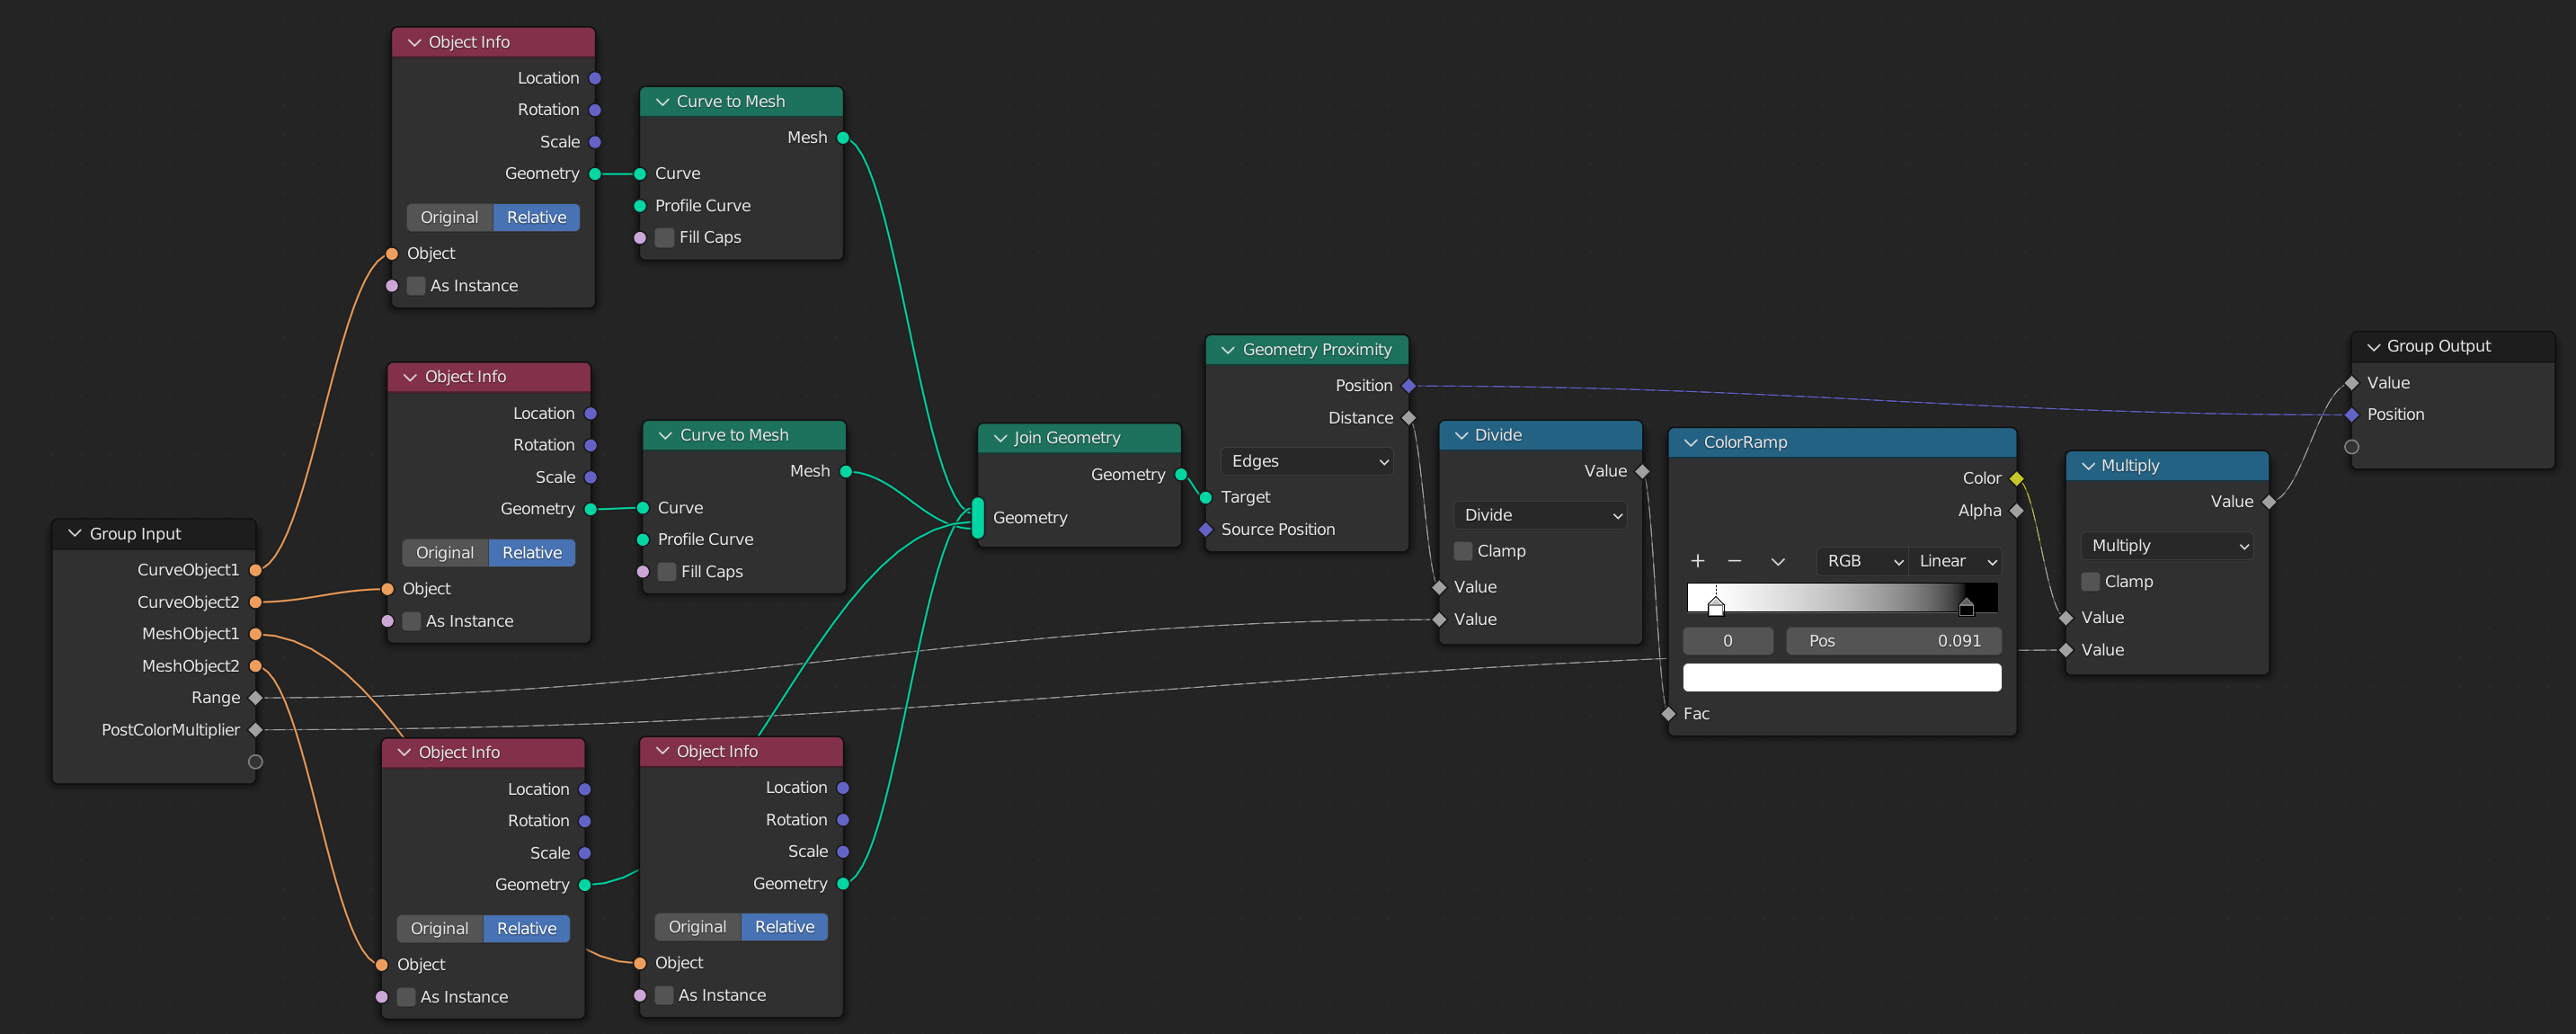
\includegraphics[width=14.5cm]{src/img/pic/pic-3 blender geometry screenshot curve_distance.png}
    \caption{Geometry Node Implementation for curve_distance}
    \label{fig:impl-curve-dist}
\end{figure}

\begin{figure}[H]
    \centering
    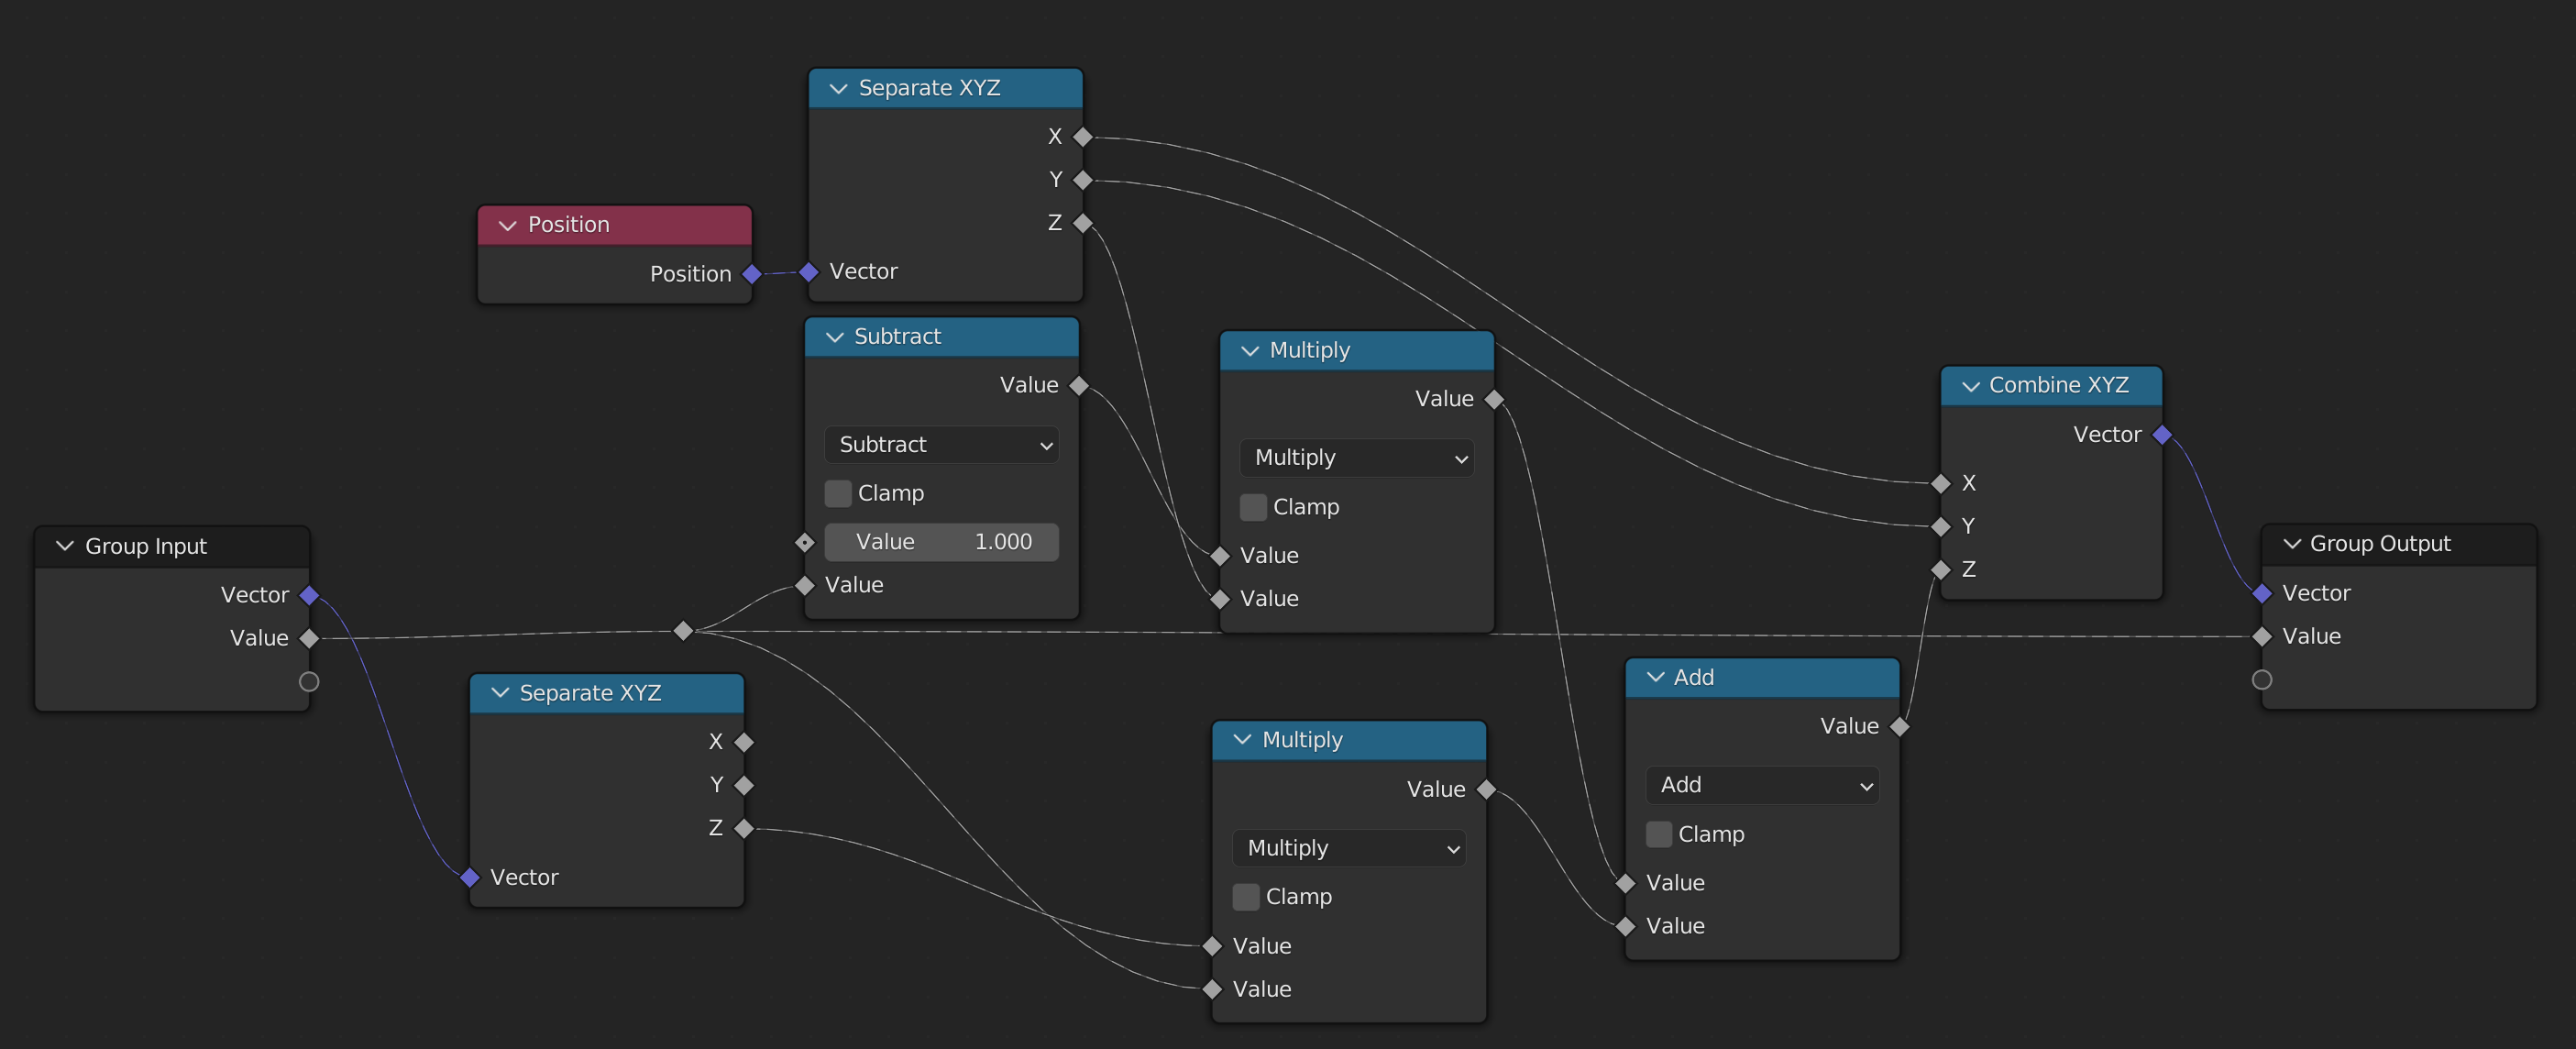
\includegraphics[width=14.5cm]{src/img/pic/pic-4 blender geometry node screenshot adjust_z_to_match_pos.png}
    \caption{Geometry Node Implementation for adjust_z_to_match_pos}
    \label{fig:impl-adjust-z-to-match-pos}
\end{figure}


TODO Some text here for latex placement


% ###############################################################
\section{Procedural Railway Generation}
\label{sec:procedural-railway-generation}

TODO planks

TODO rails

TODO signage



% ###############################################################
\section{Vegetation Scatter and Geometry Caching}
\label{sec:vegetation-scatter}


TODO veg


% ###############################################################
\section{Scene Setup and Rendering Loop}
\label{sec:rendering}


TODO render loop / interactive
